Interest in opinion of other individuals is probably as old as the communication itself. There is evidence that already in ancient Greece, generals were trying to detect dissent among their subordinates using various "primitive" approaches \cite{richmond1998spies}. Another approach to measure and evaluate a public opinion coming from ancient Greece and used to these date is voting. In the first decades of twentieth century, efforts in capturing public opinion started utilize questionaires and in 1937, first scientific journal on public opinion was founded. 

In the last 10 years, SE and ML in general experienced a big boom. According to data collected by Mantyla, Graziotin and Kuutila \cite{mantyla2018evolution}, nearly 7000 papers about sentiment analysis have already been written and not surprisingly, 99\% of them were published after 2004 - making sentiment analysis one of the fastest growing research areas. The increasing interest about this area can be seen in the figure \ref{fig:papersCountHistory}.

\begin{figure}[H]%
    \centering
	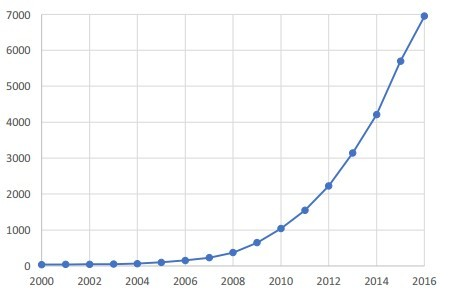
\includegraphics[width=8cm]{papersCountHistory.jpg}
    \caption{Cumulative count of papers about sentiment analysis \cite{mantyla2018evolution}}%
    \label{fig:papersCountHistory}%
\end{figure}

